\section{Decomposition 1: Av3, UC14, UC15, UC18 (SIoTIP System)}


\subsection*{Selected architectural drivers}
    The non-functional drivers for this decomposition are:
    \begin{itemize}
    	\item \emph{Av3}: Pluggable device or mote failure
    \end{itemize}

    The related functional drivers are:
    \begin{itemize}
    	\item \emph{UC14}: Send heartbeat (Av3) \\
              This use case checks whether or not motes and pluggable devices
              are still operational.
    	\item \emph{UC15}: Send notification (Av3) \\
              This use case sends a notification to a registered user.
    	\item \emph{UC18}: Check and deactivate applications (Av3) \\
              This use case deactivates any application that requires deactivation,
              because of unavailability of essential pluggable devices
              or unassigned mandatory roles.
    \end{itemize}

    \paragraph{Rationale}
        Av3 was chosen first since it has high priority and it is more relevant to
        the core of the system than the other quality requirements with high
        priority (M1 and U2).
        We believe that handling pluggable device failure/connectivity is
        more important to the whole of the system than M1 and U2, and that
        handling this first would give a stronger starting point for later ADD iterations
        than M1 or U2.


\subsection*{Architectural design}\label{sec:architectural-design}
    This section describes what needs to be done to satisfy the requirements for
    this decomposition and how involved problems/obstacles are solved.

    \paragraph{Av3: Failure detection}
        Gateway need to be able to autonomously detect failure of one of its
        connected motes and pluggable devices. This is achieved by making motes
        send heartbeats to their connected gateways. The gateways can
        then monitor their connected devices. The heartbeats contain a list
        of devices that are connected/operational at the moment the mote sends
        the heartbeat. Each gateway makes use of a \texttt{DeviceManager}
        component to monitor the devices. This component uses timers to keep track
        of how long it has been since a device has sent a heartbeat or occured in
        a list of connected devices. Once a timer expires, this is treated as
        a failure. \\

        A mote has failed when 3 consecutive heartbeats do not arrive within 1
        second of their expected arrival time. \\
        A pluggable device has failed when it does not occur in a heartbeat of the
        mote in which it is expected to be in. This is is detected within 2
        seconds after the arrival of the heartbeat.

    \paragraph{Av3: Automatic application deactivation and redundancy settings}
        Applications should be automatically suspended when they can no longer
        operate due to failure of a pluggable device or mote and reactivated
        once the failure is resolved. Application providers can design their
        applications such that they explicitly require redundancy in
        the available pluggable devices. \\
        This problem is tackled by the \texttt{DeviceManager}. It
        stores the requirements for pluggable devices set by applications for all
        applications that use the gateway that the the \texttt{DeviceManager}
        runs on. When it detects that an application can no longer operate
        due to failures, it will send a command to the \texttt{ApplicationManager}
        (via the \texttt{GatewayFacade})
        to suspend that application. When the required devices are operational
        again, the \texttt{DeviceManager} detects this and sends a
        command to reactivate the application. \\

        Applications are suspended within 1 minute after detecting
        the failure of an essential pluggable device. \\
        Application are reactivated within 1 minute after the failure is resolved.

    \paragraph{Av3: Notifications}
        The infrastructure owner should be notified of any persistent
        pluggable device or mote failures. Customer organisations should be
        notified if one or more of their applications is suspended or
        reactivated. Applications using a failed pluggable device or any device
        on a failed mote should be notified. \\
        The \texttt{NotificationHandler} was put in place to deal with
        notifications. Other components can use it to generate notifications for
        certain users in the system. The \texttt{NotificationHandler} will then
        insert information relevant to the notification in the database (message,
        status, date and time, source, ...), and use an external delivery
        service to deliver the notification to users. The used delivery medium
        is based on the user's preferences. \\
        Since they are stored in the database, users can always view
        their notifications via their dashboard. However, this funcionality is not
        expanded on in this decomposition yet. \\

        Infrastructure owners are notified within 1 minute after detecting a mote outage lasting at
        least 10 seconds. \\
        Infrastructure owners are notified within 1 minute after the detection of the unavailability of
        a pluggable device for 30 seconds. \\
        Applications are notified of the failure of relevant pluggable devices within 10 seconds.

    \subsubsection{Alternatives considered}
        \paragraph{Av3: Failure detection}
            An alternative would have been to move the \texttt{DeviceManager}
            component from gateways to the Online Service. This solution would make the
            gateways do less work, but would be very unscalable. The reason is
            that as the customer base (and thus the amount of devices) increases,
            the Online Service would need to keep track of huge amounts of devices.
            This would also flood the network to the Online Service with heartbeats.

        \paragraph{Av3: Failure detection}
            Another alternative for failure detection could have been the use of
            a Ping/Echo mechanism instead of Heartbeats. Pings could then be used
            to check if a device is currently operational. However, as a device could
            not be operational for a moment because of e.g. interference, timers
            would still be necessary to keep track of operational devices. We opted
            to use heartbeats, as this would reduce the amount of data sent over
            the network used by the motes, and as motes would have to do slightly
            more work to process each Ping request in order to generate a reply.

        \paragraph{Av3: Notifications}
            Reliable and quick delivery of notifications is crucial to the
            system in order to solve problems should things go wrong. Currently,
            the solution is to use a third party service for delivery of
            notifications. In the case that no external services are found
            satisfactory, or if this dependency on an external service is
            unwanted, it is possible to build an internal solution for this.
            For example, a \texttt{NotificationSender} component could make use
            of the \texttt{Factory pattern} for different message channels for
            different delivery methods (each with their own sendNotification method).
            This solution allows us to easily add new message channels in the
            future with little effort. The disadvantage of this is that an
            internal solution takes a lot more time to implement.


\subsection*{Instantiation and allocation of functionality}
    This section lists the new components which instantiate our solutions
    described in the section above. For each component we note the quality
    attribute or use case that prompted us to create it. Descriptions about
    the components can be found under chapter \ref{ch:elements-datatypes}. \\

    \begin{itemize}
        \item ApplicationManager: Av3
        \item Database: /
        \item DeviceManager: Av3
        \item GatewayFacade: /
        \item Mote: UC14
        \item NotificationHandler: UC15
    \end{itemize}

    \paragraph{Decomposition}
        Figure \ref{fig:it1-cc_main} shows the components resulting from the
        decomposition in this run.

        \begin{figure}[!htp]
        	\centering
        	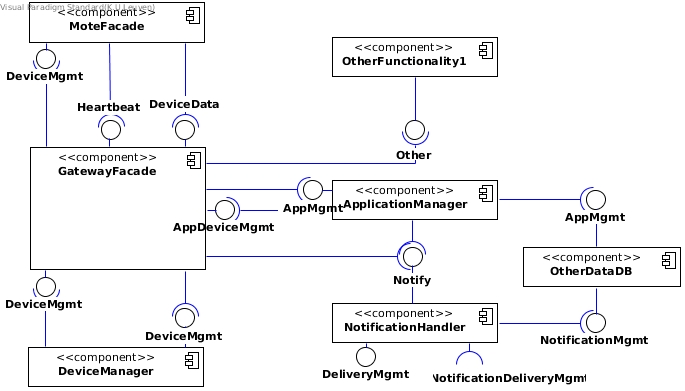
\includegraphics[width=1.00\textwidth]{images/component-diagram-1}
        	\caption{Component-and-connector diagram of this decomposition.}
            \label{fig:it1-cc_main}
        \end{figure}

    \paragraph{Deployment}
        Figure \ref{fig:it1-depl_main} shows the allocation of components
        to physical nodes.

        \begin{figure}[!htp]
        	\centering
        	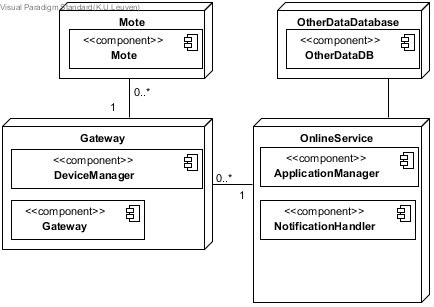
\includegraphics[width=0.55\textwidth]{images/deployment-diagram-1}
        	\caption{Deployment diagram of this decomposition.}\label{fig:it1-depl_main}
        \end{figure}


\subsection*{Interfaces for child modules}\label{add1-interfaces}
    This section lists new interfaces assigned to the components defined
    in the section above. Detailed information about each interface and
    its methods can be found under chapter \ref{ch:elements-datatypes}.

    \subsubsection{ApplicationManager}
        \begin{itemize}
            \item GWAppInstanceMgmt
        \end{itemize}

    \subsubsection{Database}
        \begin{itemize}
            \item NotificationMgmt
            \item AppMgmt
        \end{itemize}

    \subsubsection{GatewayFacade}
        \begin{itemize}
            \item Heartbeat
            \item DeviceData
            \item DeviceMgmt
            \item AppDeviceMgmt
        \end{itemize}

    \subsubsection{Mote}
        \begin{itemize}
            \item DeviceMgmt
        \end{itemize}

    \subsubsection{NotificationHandler}
        \begin{itemize}
            \item Notify
            \item DeliveryMgmt
        \end{itemize}

    \subsubsection{External notification delivery service}
        \begin{itemize}
            \item NotificationDeliveryMgmt
        \end{itemize}

    \subsubsection{DeviceManager}
        \begin{itemize}
        	\item DeviceMgmt
        \end{itemize}


\subsection*{New data types}
    This section lists the data types introduced in this decomposition.

    \begin{itemize}
        \item{PluggableDeviceInfo}
        \item{Notification}
        \item{ApplicationInstance}
        \item{Subscription}
        \item{PluggableDeviceID}
        \item{PluggableDeviceType}
        \item{DeviceData}
        \item{Map<String,String>}
    \end{itemize}

\subsection*{Verify and refine}
    The selected architectural drivers have been handled completely
    in this decomposition.
    This section describes per component which (parts of) the remaining
    requirements it is responsible for. If requirements are split in
    multiple parts, this is indicated by the addition of a letter
    (or number, depending on the structure of the requirement) after their title.

    \paragraph{ApplicationManager}
        \begin{itemize}
            \item \emph{Av2}: Application failure \\
                   Prevention: a, b \\
                   Detection: a, b, c \\
                   Resolution: a, b, c
           \item \emph{P1}: Large number of users: c
           \item \emph{M1}: Integrate new sensor or actuator manufacturer: 1.c, 2.a
           \item \emph{M2}: Big data analytics on pluggable data and/or application usage data: d, e
           \item \emph{U1}: Application updates: a, b, c, d
           \item \emph{U2}: Easy Installation: e
           \item \emph{UC12}: Perform actuation command
           \item \emph{UC17}: Activate an application: 3, 4
        \end{itemize}

    \paragraph{Database}
        \begin{itemize}
          	\item None
        \end{itemize}

    \paragraph{GatewayFacade}
        \begin{itemize}
            \item \emph{Av1}: Communication between SIoTIP gateway and Online Service \\
                              Resolution: b, c, d
            \item \emph{M1}: Integrate new sensor or actuator manufacturer: 1.a, 2.b
            \item \emph{U2}: Easy Installation: a, c, d
            \item \emph{UC11}: Send pluggable device data: 1
        \end{itemize}

    \paragraph{Mote}
        \begin{itemize}
            \item \emph{M1}: Integrate new sensor or actuator manufacturer: 1.a, 2.b
            \item \emph{U2}: Easy Installation: b, c, d
            \item \emph{UC04}: Install mote: 1, 2
            \item \emph{UC05}: Uninstall mote: 1
            \item \emph{UC06}: Insert a pluggable device into a mote: 2
            \item \emph{UC07}: Remove a pluggable device from its mote: 2
            \item \emph{UC11}: Send pluggable device data: 1
        \end{itemize}

    \paragraph{NotificationHandler}
        \begin{itemize}
            \item \emph{UC16}: Consult notification message: 5
            \item \emph{UC17}: Activate an application: 5, 6
        \end{itemize}

    \paragraph{OtherFunctionality1}
        \begin{itemize}
            \item \emph{Av1}: Communication between SIoTIP gateway and Online Service \\
                               Detection: a, b, c, d
                               Resolution: a
           	\item \emph{P1}: Large number of users: a
            \item \emph{P2}: Requests to the pluggable data database
            \item \emph{M1}: Integrate new sensor or actuator manufacturer: 1.d
            \item \emph{M2}: Big data analytics on pluggable data and/or application usage data: a
            \item \emph{U2}: Easy Installation: e
            \item \emph{UC01}: Register a customer organisation
            \item \emph{UC02}: Register an end-user
            \item \emph{UC03}: Unregister an end user
            \item \emph{UC04}: Install mote: 3
            \item \emph{UC05}: Uninstall mote: 2.b
            \item \emph{UC06}: Insert a pluggable device into a mote: 3: topology part; alternative 3a.1.b
            \item \emph{UC07}: Remove a pluggable device from its mote: 3.b
            \item \emph{UC08}: Initialise a pluggable device: 1, 2, 4
            \item \emph{UC09}: Configure pluggable device access rights
            \item \emph{UC10}: Consult and configure the topology
            \item \emph{UC11}: Send pluggable device data: 3
            \item \emph{UC13}: Configure pluggable device
            \item \emph{UC16}: Consult notification message: 1, 2, 3, 4
            \item \emph{UC17}: Activate an application: 1, 2
            \item \emph{UC19}: Subscribe to application
            \item \emph{UC20}: Unsubscribe from application
            \item \emph{UC21}: Send invoice
            \item \emph{UC22}: Upload an application
            \item \emph{UC23}: Consult application statistics
            \item \emph{UC24}: Consult historical data
            \item \emph{UC25}: Access topology and available devices
            \item \emph{UC26}: Send application command or message to external front-end
            \item \emph{UC27}: Receive application command or message to external front-end
            \item \emph{UC28}: Log in
            \item \emph{UC29}: Log out
        \end{itemize}

    \paragraph{DeviceManager}
        \begin{itemize}
            \item \emph{U2}: Easy Installation: c, d
            \item \emph{UC04}: Install mote: 4
            \item \emph{UC05}: Uninstall mote: 2
            \item \emph{UC06}: Insert a pluggable device into a mote: 3: uninitialised part; alternative 3a.1 3a.2 3a.4; 4
            \item \emph{UC07}: Remove a pluggable device from its mote: 3.a, 3.c
            \item \emph{UC08}: Initialise a pluggable device: 3
            \item \emph{UC11}: Send pluggable device data: 2, 3a
        \end{itemize}
